%%%% Proceedings format for most of ACM conferences (with the exceptions listed below) and all ICPS volumes.
\documentclass[sigconf]{acmart}
%%%% As of March 2017, [siggraph] is no longer used. Please use sigconf (above) for SIGGRAPH conferences.

%%%% Proceedings format for SIGPLAN conferences 
% \documentclass[sigplan, anonymous, review]{acmart}

%%%% Proceedings format for SIGCHI conferences
% \documentclass[sigchi, review]{acmart}

%%%% To use the SIGCHI extended abstract template, please visit
% https://www.overleaf.com/read/zzzfqvkmrfzn


\usepackage{booktabs} % For formal tables
\usepackage[utf8x]{inputenc}

% Copyright
% \setcopyright{none}
%\setcopyright{acmcopyright}
%\setcopyright{acmlicensed}
%\setcopyright{rightsretained}
%\setcopyright{usgov}
%\setcopyright{usgovmixed}
%\setcopyright{cagov}
%\setcopyright{cagovmixed}


% DOI
\acmDOI{10.475/123_4}

% ISBN
\acmISBN{123-4567-24-567/08/06}

%Conference
%\acmConference[WOODSTOCK'97]{ACM Woodstock conference}{July 1997}{El
 % Paso, Texas USA}
%\acmYear{1997}
%\copyrightyear{2016}


\acmArticle{4}
%\acmPrice{15.00}

% These commands are optional
%\acmBooktitle{Transactions of the ACM Woodstock conference}



\begin{document}
\title{Uma proposta de ontologia para PEP com foco na resolução de problemas de interoperabilidade e gerenciamento de triagem em atenção básica de saúde}



\author{Igor Roberto Guilherme}
\affiliation{%
  \institution{Universidade de São Paulo}
  \streetaddress{P.O. Box 1212}
  \city{São Carlos}
  \state{São Paulo}
  \postcode{43017-6221}
}
\email{igor.guilherme@usp.br}


\begin{abstract}
Prontuários Eletrônicos do Paciente (PEP) são cada vez mais utilizados, pois minimizam os riscos presentes nos prontuários de papel, como a segurança e o extravio. Porém, observa-se que no Brasil cada unidade de saúde tem a autonomia de desenvolver seu próprio PEP, causando problemas de interoperabilidade por conta da falta de padrão adotada. A falta interoperabilidade no domínio da saúde, dificulta que sejam criados sistemas de auxílio, como os Sistemas de Apoio a Decisão. Desta forma, o presente trabalho se propõe a elaboração de uma ontologia para PEP, que tenhas os elementos necessários para que se identifique sua criticidade. Posteriormente, o desenvolvimento de um protótipo que utilize a ontologia e gerencie a triagem de acordo com a criticidade de cada prontuário.   
 \end{abstract}

%
% The code below should be generated by the tool at
% http://dl.acm.org/ccs.cfm
% Please copy and paste the code instead of the example below.
%


\keywords{Ontologia, Saúde, Prontuário, Triagem}


\maketitle

\section{Introdução}

O conhecimento na área da saúde é baseado em dados coletados de pesquisas experimentais clínicas, epidemiológicas e da prática profissional em saúde. Desta forma, os dados são provenientes de enumeras fontes, dificultando a gestão, análise e tomada de decisão com a interpretação destes dados. Há algumas iniciativas globais que buscam resolver problemas relacionados a troca de informações clínicas, entre sistemas de saúde. Algumas organizações como HL7 e OpenEHR que buscam criar ferramentas e padrões com o fim de prover mecanismos para resolução de problemas de interoperabilidade. Um outro problema na área da saúde, é a triagem do paciente para o encaminhamento a serviços especializados, procedimento realizado muitas vezes de forma manual. Atenção Básica é a terminologia utilizada no país e internacionalmente para denominar Atenção Primária à Saúde(APS). Logo, a APS funciona como elemento de ordenamento dos fluxos e contra-fluxos de pessoas, produtos e informações nas redes, dialogando com as atenções secundárias e terciárias através da regulação assistencial.\cite{Nayara}
O ministério da saúde, disponibiliza o sistema Sistema Nacional de Regulação (SISREG) para que os municípios possam regulamentar e fazerem a  gestão das listas de espera. Este sistema não tem caráter compulsório, portanto cada município pode realizar a gestão de fila utilizando os próprios critérios.\cite{SISREG} Algumas unidades básicas de saúde (UBS) realizam a triagem dos pacientes para um atendimento mais especifico utilizando o Sistema de Triagem de Manchester, que se mostra um bom preditor para desfechos clínicos. \cite{TRIAGEMAVALICAO} 


\section{Prontuário }

A palavra prontuário deriva do latim promptuariu que significa lugar onde se guarda aquilo que deve estar à mão, o que pode ser necessário a qualquer momento\cite{PATRICIO}. De acordo com a resolução nº 1.638/2002 do Conselho Nacional de Medicina, o prontuário é um documento único constituído de um conjunto de informações, sinais e imagens registradas, geradas a partir de fatos, acontecimentos e situações sobre a saúde do paciente e a assistência a ele prestada. A mesma resolução considera que o médico tem o dever de elaborar o prontuário para cada paciente a que assiste, conforme previsto no Código de Ética de medicina. A denominação de "Prontuário Médico" foi substituída por "Prontuário do Paciente", devido ás transformações na relação médico-paciente, com ênfase na defesa dos direitos dos pacientes.\cite{PATRICIO} 

O prontuário é uma peça fundamental no atendimento clínico, pois através dos registros, permite analisar a evolução do estado do paciente, além de possibilitar uma pós-análise dos eventos registrados.
Segundo Marin\cite{MARIN}, Hipócrates no século V a.C, solicitava aos médicos a elaboração de registros escritos para avaliar a evolução da enfermidade e identificar suas possíveis causas. 

Prontuários de papel ainda são utilizados hoje em dia, seja por problemas financeiros das unidades de saúde para a implantação de um sistema, ou até mesmo por conta do comodismo da gestão dessa unidades em dotar um novo procedimento. Todavia, esses documentos tem o eminente risco de quebra de privacidade e de extravio das informações. Existe, ainda, a dificuldade para recuperação de informações importantes para tomada de decisão e/ou que devem ser compartilhadas entre os profissionais de saúde e com os pacientes.\cite{SALVADOR}

\subsection{PRONTUÁRIO ELETRÔNICO}

Com potencial para otimizar a eficiência e efetividade dos serviços de saúde, o prontuário eletrônico do paciente (PEP) tem se destacado como uma importante ferramenta no gerenciamento dos serviços de saúde
\cite{GONCALVES}.  Há mais de duas décadas, os avanços tecnológicos trouxeram uma nova tendência aos prontuários - em pequenos e grandes centros de saúde, públicos e privados - e estimularam os serviços de saúde a utilizarem, cada vez mais, um Sistema de Registro Eletrônico em Saúde (S-RES), direcionando os esforços para a demanda dos novos modelos de atenção à saúde, fomentada pela Organização Mundial da Saúde (OMS) \cite{Downing}. Nos próximos anos os prontuários eletrônicos dos pacientes (PEP) terão papéis cada vez mais importantes na prestação de serviços de saúde, particularmente na criação de novas oportunidades para melhorar a qualidade e eficácia.\cite{Downing}

A estrutura de um prontuário, independente de ser eletrônico ou em papel, deve seguir as orientações e determinações da Resolução CFM Nº 1638/2002 que define prontuário médico e torna obrigatória a criação da Comissão de Revisão de Prontuários nas instituições de saúde.\cite{SIBIS}A mesma resolução ainda prevê que todo prontuário deve obrigatoriamente conter a identificação do paciente, anamnese, exame, hipóteses diagnósticas, diagnósticos definitivos e tratamentos efetuados. Apesar de haver algumas determinações pelos órgãos que realizam a gestão da saúde no Brasil, cada unidade de saúde pode utilizar um sistema próprio de prontuário eletrônico, causando problemas de interoperabilidade entre esses sistemas, o que acaba dificultado a criação de sistemas que utilizes esses dados para auxilio no atendimento médico.

O Ministério da Saúde oferece gratuitamente o e-SUS AB, que é um sistema de prontuário eletrônico para a atenção básica, mas os municípios podem optar por desenvolver ou utilizar seus sistemas próprios. Atualmente apenas 35\% das UBS, enviam dados por meio do Prontuário Eletrônico ao governo federal \cite{DATASUS}. No final de 2016, o Ministério da saúde exigiu que os municípios utilizassem o e-SUS AB ou sistema próprio para prontuário eletrônico ou então justificassem suas limitações, e foi obtido o seguinte resultado como alegação \cite{DATASUS2016}:
  \begin{itemize}
        	\item 84,9\% (21.205 UBS) - insuficiência de equipamentos
        	\item 73,9\% (18.493) - conectividade
        	\item 75\% (18.750) - baixa qualificação no uso do Prontuário Eletrônico
        	\item 67,9\% (16.989) - falta de apoio de Tecnologia da Informática
        	\item As cidades que não justificaram tiveram suspensos os recursos destinados ao custeio dos atendimentos na Atenção Básica (PAB Variável)
 \end{itemize}
\section{Interoperabilidade}
	Na área da computação, interoperabilidade é definida como a característica de um produto ou sistema, os quais as interfaces são completamente compreendidas, são capazes de interagir com outros sistemas no presente momento ou no futuro, sem nenhuma restrição \cite{CHAPURLAT20121523}.
	A interoperabilidade é divida em sete tipos, segundo  Ukoln (2005):
    \begin{itemize}
        	\item Interoperabilidade técnica: abrange padrões de comunicação, de transporte,
de armazenamento e de representação de informações.
            \item Interoperabilidade semântica: refere-se ao significado da informação originada
em diferentes sistemas. 
            \item Interoperabilidade organizacional: relacionada ao contexto organizacional,
busca alinhamento entre processos e informações presentes na arquitetura
corporativa. 
            \item Interoperabilidade política e humana: envolve a forma como a informação é
disseminada, ou se torna disponível na organização.
            \item Interoperabilidade intercomunitária: aborda o acesso a informações originadas
em diferentes fontes, por organizações, especialistas e comunidades de
natureza distintas. 
\item Interoperabilidade legal: relacionada a exigências e implicações legais de
tornar a informação livre e amplamente disponível. 
\item  Interoperabilidade internacional: envolve a cooperação em escala
internacional, onde o intercâmbio envolve uma grande diversidade de padrões
e normas, além de problemas inerentes de comunicação por barreiras
linguísticas. 

        \end{itemize}
    Segundo (HIMSS, 2013) \cite{HIMSS} A interoperabilidade semântica é nível mais alto e diz respeito a habilidade de dois ou mais sistemas/elementos de trocar informações e utilizá-las. Apoia-se na estrutura da troca de dados e na codificação de dados, incluindo vocabulário.
    O objetivo da interoperabilidade semântica é criar um padrão semântico que seja capaz de traduzir ou integrar os vocabulário A e B em um vocabulário C, de forma que as fontes 1 e 2 sejam capazes de compreender uma a outra\cite{INTEROPENEHR}. Conforme a figura 1.    
        
 \begin{figure}[htbp]
    	\centering
        \caption{A proposta da interoperabilidade semântica.}
        \label{fig:mapeamento-ontologia.png}
        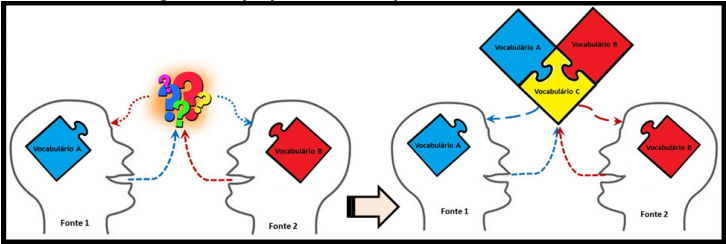
\includegraphics[width=1\linewidth]{mapeamento-ontologia.png}
        Fonte: FARINELLI, F.; ALMEIDA, M.B.(2014)
\end{figure}

\subsection{Interoperabilidade no contexto da saúde}
Dentre as diversas aplicações das Tecnologias da Informação e Comunicação (TIC) que desempenham recursos para facilitar a criação e o uso de dados, de informação e de conhecimento de saúde; a Interoperabilidade surge como a capacidade que os diversos sistemas da informação e aplicativos de software têm de se comunicar, trocar dados e utilizar as informações trocadas para suportar e viabilizar todos os aspectos do sistema de saúde\cite{SCIARRA}. Ainda para Adília e João(2018)\cite{SCIARRA},  o setor da saúde no Brasil ainda guarda muitos desafios, entre eles o próprio uso da Tecnologia da Informação (TI). Nesse aspecto, a Interoperabilidade já está deixando de ser uma tendência para ser uma exigência do mercado, uma vez que, além de reduzir custos e eliminar deficiências através da automatização de tarefas, oferece maior controle e agilidade do workflow e otimização do tempo; garante também ao paciente uma melhor experiência de atendimento. 
    No domínio da saúde existem alguns padrões estabelecidos com o objetivo de resolver problemas de interoperabilidade. Tais como OpenEHR que é uma arquitetura para criar Registros Eletrônicos em Saúde(RES) interoperáveis e independentes da tecnologia utilizada para sua captura, o  HL7 RIM que possibilita a interoperabilidade semântica ao fornecer um vocabulário padrão e mensagens estruturadas em XML.
\subsection{Padrões no Brasil}
No Brasil, a portaria nº 3.947 de 25 de novembro de 1998, estabeleceu  a utilização da Classificação Internacional
de Doenças (CID), proposta pelo Organização Mundial da Saúde (OMS) para a causa do atendimento e para o diagnóstico e a tabela
unificada do SUS para os procedimentos realizados \cite{BRASIL1998}.
A portaria nº 2.073, de 31 de agosto de 2011 estabelece um catálogo de padrões de informação, entre eles algumas terminologias e ontologias: SNOMEDCT,
LOINC, CID-10, TUSS e a Tabela de Procedimentos SUS. Esta última classifica os procedimentos médicos em grupos e subgrupos, atribuindo-os códigos e descrições. Estabelece ainda o HL7 como padrão para a troca de mensagens entre sistemas referentes a solicitações de exames e envio de resultados. \cite{BRASIL2011}.

Um dos padrões de dados que se destaca na área da saúde é a Systematized Nomenclature of Medicine Clinical Terms - SNOMED CT - (Nomenclatura Sistematizada da Medicina) \cite{BARRA}. Para determinar um diagnóstico, a SNOMED, utiliza
codificações de vários eixos (topográfico, morfológico, organismo vivo e funcional) a exemplo do diagnóstico de pneumonia pneumocócica (D-13510)  que é composta do código para o eixo tomográfico T-28000 (pulmão), no eixo morfológico por M-40000 (inflamação) e pelo eixo de Organismos Vivos L-25116 (Streptococcus pneumoniae), conforme apresentado na Figura 2 \cite{MIRANDA} .

\begin{figure}[htbp]
    	\centering
        \caption{Demonstrativo}
        \label{fig:exemplo-snomed.png}
        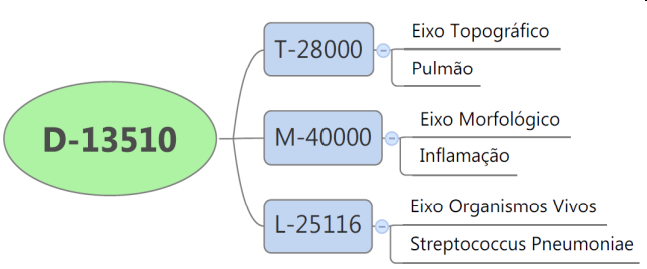
\includegraphics[width=1\linewidth]{exemplo-snomed.png}
        Fonte: MIRANDA(2015)
\end{figure}

\section{Ontologias}
Ontologias são utilizadas para representar o conhecimento, correlacionando conceitos de um domínio. Na Web Semântica, as ontologias exercem um papel fundamental na confecção de um meio de descrição do conhecimento de especialistas de um domínio. Apesar do conceito de ontologia ser aplicável em vários campos, eles urgiu primeiro no ramo da filosofia, onde se refere ao estudo da realidade do ser, da natureza e das suas relações.\cite{HOFWEBER}

 \begin{figure}[htbp]
    	\centering
        \caption{Níveis de representação de dados.}
        \label{fig:nivel-dados.png}
        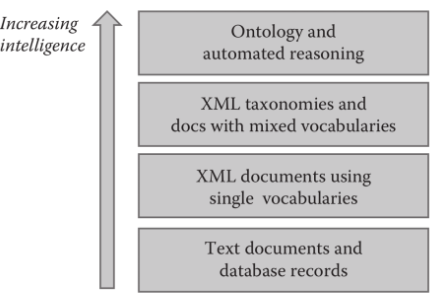
\includegraphics[width=1\linewidth]{nivel-dados.png}
        Fonte:  Allemang e Hendler (2011) 
\end{figure}



Dos níveis de representação de dados, ontologia é o mais alto por permitir inferências a partir de algumas definições. Como os conceitos de um domínio estão correlacionados através de triplas: sujeito, predicados e objetos, é possível interpretar essas relações e fazer deduções, ampliando a semântica.
Ontologias podem desempenhar papel relevante
na busca pela interoperabilidade semântica entre sistemas\cite{INTEROPENEHR}. Não foi encontrada na literatura uma ontologia que abordasse todo o Prontuário Eletrônico, apenas segmentos, devido ao grande volume de elementos que seriam necessários para o descrever em todos os cenários.
\section{Proposta}

O presente trabalho pretende analisar as principais terminologias e ontologias existentes que são utilizadas com o intuito de interoperar sistemas clínicos e elaborar uma nova ontologia voltada para o Prontuário Eletrônico do Paciente(PEP) que una as existentes a fim de possibilitar que sistemas interpretem dados semânticos e auxiliem profissionais da área da saúde no atendimento dos pacientes.
Por fim, essa ontologia deverá ser validada por médicos, como forma de garantir que o projeto elaborado representa as relações e conceitos existentes no domínio da saúde. Ainda, como forma de comprovar a utilidade da ontologia será elaborado um protótipo que gerencie a triagem dos pacientes da rede básica de saúde de acordo com a criticidade de cada prontuário.



\section{Conclusão}
Como este artigo é apenas uma apresentação do projeto que será elaborado, ainda não se tem resultados que possam aqui ser mencionados. Desta forma, a conclusão fica limitada a enfatizar a proposta da elaboração de uma ontologia para prontuário eletrônico do paciente. Como forma de não se desenvolver um trabalho muito extenso, a ontologia será segmentada nas características de um prontuário para que se possa saber seu nível de criticidade, e assim desenvolver um protótipo que analise e elabore uma triagem automatizada. Pretende-se que a ontologia utilize terminologias existentes na área da saúde, afim de obter termos e conceitos já bem estruturados e validados. Fica claro, que há a necessidade de se explorar este campo da ciência, de acordo com a pesquisa realizada onde alguns autores como (FARINELLI e ALMEIDA, 2014)\cite{INTEROPENEHR} dizem que muito ainda
está por ser feito para que a possibilidade da interoperabilidade semântica em aplicações de saúde se torne real.
%\end{document}  % This is where a 'short' article might terminate






\bibliographystyle{ACM-Reference-Format}
\bibliography{sample-bibliography}

\end{document}
